%%%%%%%%%%%%%%%%%%%%%%%%%%%%%%%%%%%%%%%%%%%%%%%%%%%%%%%%%%%%%%%%%%%%%%%%
%                                                                      %
%     File: Thesis_Implementation.tex                                  %
%     Tex Master: Thesis.tex                                           %
%                                                                      %
%     Author: Andre C. Marta                                           %
%     Last modified :  4 Mar 2024                                      %
%                                                                      %
%%%%%%%%%%%%%%%%%%%%%%%%%%%%%%%%%%%%%%%%%%%%%%%%%%%%%%%%%%%%%%%%%%%%%%%%

\chapter{Numerical Setup}
\label{chapter:numerical_setup}

In this chapter, we will describe the numerical setup of the \texttt{bamps} code. We will start by discussing the grid setup in section \ref{section:grid}, followed by the numerical method used to solve the partial differential equation systems in section \ref{section:Numerical_Method}. Finally, we will discuss the adaptive mesh refinement (AMR) strategy employed in \texttt{bamps} in section \ref{section:amr}.

%%%%%%%%%%%%%%%%%%%%%%%%%%%%%%%%%%%%%%%%%%%%%%%%%%%%%%%%%%%%%%%%%%%%%%%%
\section{Grid Setup}
\label{section:grid}

The \texttt{bamps} code uses a multi-patch grid setup to cover the computational domain. Even though \texttt{bamps} is capable of supporting both a cubed-ball grid and a cubed-sphere grid, in this work we will only use the cubed-ball grid. The grid is composed of several patches which are shaped like deformed cubes that fit together to cover the domain. Each patch is mapped by two different coordinate systems: the local patch coordinates $(\bar{x},\bar{y},\bar{z})$ and the global Cartesian coordinates $(x,y,z)$.

The cubed-ball grid consists of a central cube surrounded by six deformed cube patches that form a spherical shell around the central cube forming a transition shell, which is itself surrounded by six more deformed cube patches that form the outer spherical shell. In the central cube, the local patch coordinates and the global Cartesian coordinates are identical, i.e., $(\bar{x},\bar{y},\bar{z}) = (x,y,z)$. However, in the other patches, a coordinate transformation must be applied to map the local patch coordinates to the global Cartesian coordinates. This transformation is perrformed in two steps: first, the local coordinates are transformed to temporary global coordinates $(\tilde{x},\tilde{y},\tilde{z})$, which are then transformed to the final global Cartesian coordinates $(x,y,z)$ by performing a rotation of the patch to their correct placement on the sphere. The transformation from local patch coordinates to temporary global coordinates is given by
%
\begin{align}
    x_t = \frac{\bar{x}}{\bar{s}} \; , \quad \quad y_t = \frac{\bar{x}}{\bar{s}} \bar{y} \; ,  \quad \quad z_t = \frac{\bar{x}}{\bar{s}} \bar{z} \; ,
\end{align}
%
where, for the outer patches,
%
\begin{align}
    \bar{s} = \sqrt{1 + \bar{y}^2 + \bar{z}^2} \; 
\end{align}
%
and for the inner patches,
%
\begin{align}
    \bar{s}(\lambda) = \sqrt{\frac{1 + 2\lambda}{1 + \lambda (\bar{y}^2 + \bar{z}^2)}} \; , \quad \quad \quad \lambda = \frac{\bar{x}^2 - \bar{x}_0^2}{\bar{x}_1^2 - \bar{x}_0^2} ,
\end{align}
%
where $\bar{x}_0$ and $\bar{x}_1$ are the boundaries of the patch in the local coordinates.

Each patch can be further divided into several subpatches, which are smaller cubes that allow for a more refined grid in specific regions of the domain. When dividing a patch into subpatches, the division is done such that subgrids of two neighboring patches match, and that neighboring patches and subpatches have the same grid-point positions on their respective boundaries. In figure \ref{fig:cubed_ball_grid}, we show an example of a cubed-ball grid divided into subpatches.

\begin{figure}[h]
    \centering
    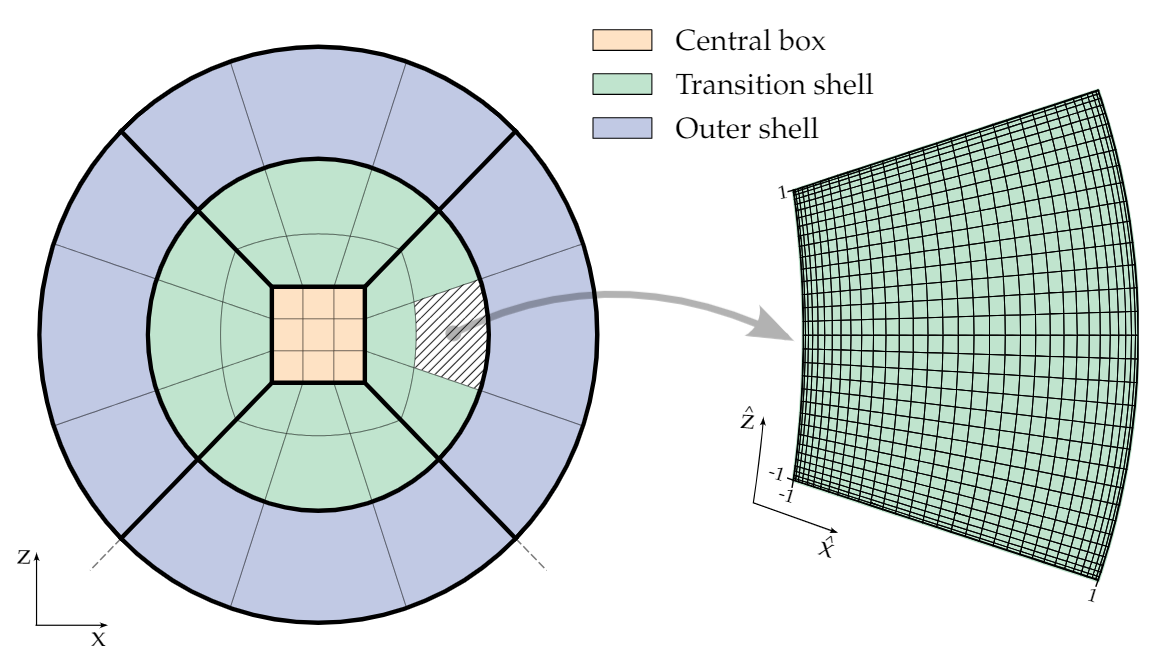
\includegraphics[width=0.8\textwidth]{Figures/Cubed_Ball.png}
    \caption{Two-dimensional sketch of the bamps cubed-ball grid layout. The grid is composed of several patches shaped like deformed cubes. These patches can be further divided into subpatches. Each subpatch is covered by Gauss-Lobatto grids.}
    \label{fig:cubed_ball_grid}
\end{figure}

%%%%%%%%%%%%%%%%%%%%%%%%%%%%%%%%%%%%%%%%%%%%%%%%%%%%%%%%%%%%%%%%%%%%%%%%
\section{Numerical Method}
\label{section:Numerical_Method}





%%%%%%%%%%%%%%%%%%%%%%%%%%%%%%%%%%%%%%%%%%%%%%%%%%%%%%%%%%%%%%%%%%%%%%%%
\section{Adaptive Mesh Refinement}
\label{section:amr}